    % \section{Local bandwidth of two synthetic example}


    % \captionsetup[subfigure]{labelformat=empty}
    % \begin{figure}[H]
    %     \centering 
    % \begin{subfigure}[b]{.48\textwidth} 
    %     \scalebox{1}{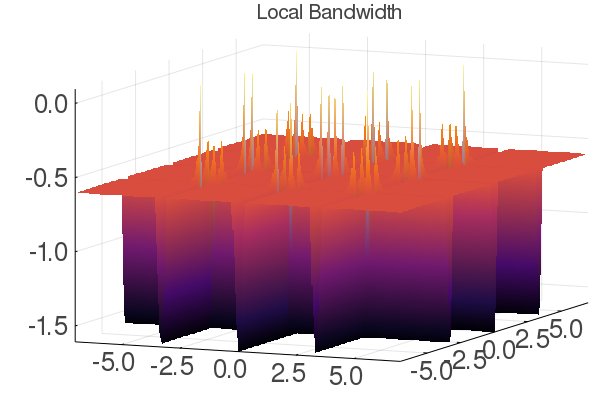
\includegraphics[width=\textwidth]{figures/bwsurf_grid.png}}
    %     \caption{(a)\label{fig:surf_grid}}
    % \end{subfigure}
    % \hfill
    % \centering
    % \begin{subfigure}[b]{0.48\textwidth}
    %     \scalebox{1}{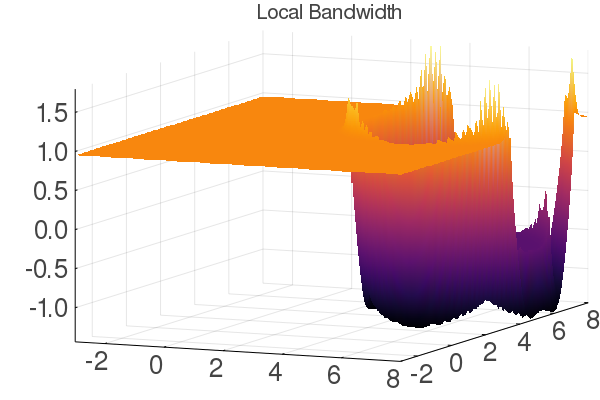
\includegraphics[width=\textwidth]{figures/bwsurf_mix.png}}
    %     \caption{(b)\label{fig:surf_mix}}
    % \end{subfigure}

    % \caption{Local bandwidth value for $4\times 4$ Gaussian grid (\cref{fig:surf_grid}) and 2-component Gaussian mixture (\cref{fig:surf_mix}).}
    % \label{fig:bwsurface}
    % \end{figure}



\section{Algorithms}

\begin{algorithm}[H] 
    \caption{SVGD} \label{alg:SVGD} 
\begin{algorithmic}
   \Procedure{SVGD}{$\{x_i^{(0)}  \}_{i = 1}^n$, $\nabla \log p(x)$, $\kappa(\cdot, \cdot)$,$\gamma_k$} 
   \For{ $k=0, 1, \dots, K-1$}
        \For{$i = 1, 2, \dots, n$}
        \State $x_{i}^{(k+1)} \leftarrow x_{i}^{(k)}+ \gamma_k \hat{\phi}_k^{\star}\left(x_{i}^{(k)}\right)$ where $\hat{\phi}_k^{\star}(\cdot)$ is defined in \cref{eq:svgd}
        \EndFor
    \EndFor
    \State \Return $\left\{x_i^{(K)}  \right\}_{i = 1}^n$ 
   \EndProcedure 
\end{algorithmic}
\end{algorithm}

\begin{algorithm}[H] 
    \caption{A-SVGD with local bandwidth} \label{alg:ASVGD_bw} 
\begin{algorithmic}
   \Procedure{SVGD}{$\{x_i^{(0)}  \}_{i = 1}^n$, $\nabla \log p(x)$, $\nabla^2 \log p(x)$,$\gamma_k$, $\alpha(t)$} 
   \For{ $k=0, 1, \dots, K-1$}
        \For{$i = 1, 2, \dots, n$}
        \State $\Sigma(x_i) \gets \text{abs}\left( \diag \left(\nabla^2 \log p(x_i) \right)^{-1}\right)$
        \State $\kappa(x, x'; \Sigma(x_i))\gets \exp(-(x - x')^T \Sigma^{-1}(x_i)(x- x')  )$
        \State $x_{i}^{(k+1)} \leftarrow x_{i}^{(k)}+ \gamma_k \hat{\phi}_{\alpha_k}\left(x_{i}^{(k)}\right)$ where $\hat{\phi}_{\alpha_k}(\cdot)$ is defined in \cref{eq:asvgd}
        \EndFor
    \EndFor
    \State \Return $\left\{x_i^{(K)}  \right\}_{i = 1}^n$ 
   \EndProcedure 
\end{algorithmic}
\end{algorithm}




\section{Details of Experiments}


\subsection{Variable transformations of Bayesian GMM} \label{supp:gmmtransformation}

To transform $(\theta_1, \dots, \theta_K) \in \Delta(K)$ and $\sigma_{kd}\in \reals_+$ into unconstrained space, we consider the change of random variables as below:
\benum
\item For $\sigma_{kd}\sim \distNamed{LogNormal}(0,1)$, we consider 
\[
     \tau_{kd} = \log(\sigma_{kd}) \sim \distNorm(0,1),   
\]
which has a full support on $\reals$.
\item For $\theta \sim \distDir(\alpha_0)$, we consider using marginalized LogGamma random variables. Notice the relationship of Gamma distribution and Dirichlet distirbution as follows, 
\[
&\left( \lambda_k\right)_{k = 1}^K \distiid \distNamed{LogGamma}(\alpha_0, 1)\\
& \left( \frac{\exp(\lambda_1)}{\sum_k \exp(\lambda_k)}, \dots, \frac{\exp(\lambda_K)}{\sum_k \exp(\lambda_k)}\right) \sim \distDir(\alpha_0),
\]
then $\lambda_k$ is supported on $\reals$. In our example, we set $\alpha_0 = 1$.
\eenum
Therefore, instead of inferring the original parameters, we perform SVGD on the posterior distribution of $(\lambda_{1:k}, \mu_{1:k}, \tau_{11:kd})$.
